%%% CMC Data Science Capstone Program
%%% Statement of Work Template
%%% Created: February 2020
%%% Updated: August 2020
%%% Modified by Jeho Park 
%%% Modified by Bhaven Mistry (Appendix Section)
%%%
%%% This SoW template is based on the work, TEAM (Teaching Experiential Action-based Materials). Materials are available at https://team-repo.github.io.
%%%
%%%%%%%%%%%%%%%%%%%%%%%%%%%%%%%%%%%%%%%%%%%%%%%%%%%
%%% Preamble (Do not change below)
%%%%%%%%%%%%%%%%%%%%%%%%%%%%%%%%%%%%%%%%%%%%%%%%%%%
\documentclass{article}
\usepackage[utf8]{inputenc}
\usepackage{url}
\usepackage{fancyhdr}
\usepackage[letterpaper, portrait, margin=1in, top=1.1in, bottom=1in]{geometry}
\usepackage[square,sort,comma,numbers]{natbib}
\usepackage{graphicx}
\usepackage{enumitem}
\usepackage{hyperref}
\hypersetup{
    colorlinks=true, % make this false if you don't want URL and ref links in color
    linkcolor=blue,
    filecolor=blue,      
    urlcolor=blue,
}

\pagestyle{fancy}
\fancyhf{}
\rhead{Statement of Work}
\lhead{CMC Data Science Capstone}
\rfoot{Page \thepage}

\newcommand{\HRule}{\rule{\linewidth}{0.5mm}} % Defines a new command for the horizontal lines, change thickness here

%%% End of Preamble (Do not change above this line)
%%%%%%%%%%%%%%%%%%%%%%%%%%%%%%%%%%%%%%%%%%%%%%%%%%%
%%%%%%%%%%%%%%%%%%%%%%%%%%%%%%%%%%%%%%%%%%%%%%%%%%%

\begin{document}

\begin{titlepage}
%%% Title page modified by Jeho Park to fit Claremont McKenna College
%%% Title page template credit:      
%%%%%%%%%%%%%%%%%%%%%%%%%%%%%%%%%%%%%%%%%
%%% Uppsala University Assignment Title Page 
%%% LaTeX Template
%%% Version 1.0 (27/12/12)
%%%
%%% This template has been downloaded from:
%%% http://www.LaTeXTemplates.com
%%%
%%% Original author:
%%% WikiBooks (http://en.wikibooks.org/wiki/LaTeX/Title_Creation)
%%% Modified by Elsa Slattegard to fit Uppsala university
%%% License:
%%% CC BY-NC-SA 3.0 (http://creativecommons.org/licenses/by-nc-sa/3.0/)
%%%%%%%%%%%%%%%%%%%%%%%%%%%%%%%%%%%%%%%%%%%%%%%%%%%

\center % Center everything on the page
 
%---------------------------------------------------------------------------------
%	HEADING SECTIONS
%---------------------------------------------------------------------------------

%\textsc{\LARGE Claremont McKenna College}\\[1.5cm] % Name of your university/college

\includegraphics[scale=.15]{cmc_logo.pdf}\\[1cm] % Include a department/university logo - this will require the graphicx package
\textsc{\Large CMC Data Science Capstone}\\[0.5cm] 
\textsc{\Large Statement of Work}\\[0.5cm] % Major heading such as course name

%---------------------------------------------------------------------------------
%	TITLE SECTION
%---------------------------------------------------------------------------------

\HRule \\[0.4cm]
{ \huge \bfseries Project Title}\\[0.2cm] % Title of your project
\HRule \\[1.0cm]

%--------------------------------------------------------------------------------
%	AUTHOR SECTION
%--------------------------------------------------------------------------------

\begin{minipage}{0.4\textwidth}
\begin{flushleft} \large
\emph{Client:}\\
NAME OF YOUR CLIENT\\[0.5cm]
\emph{Team Members:}\\
First-Name  \textsc{Last-Name}\\ % Your name
First Name  \textsc{Last Name}\\ % Your name
First Name  \textsc{Last Name}\\ % Your name
First Name  \textsc{Last Name}\\ % Your name
First Name  \textsc{Last Name}\\[0.5cm] % Your name
\emph{Faculty Advisor:}\\
First-Name  \textsc{Last-Name}\\[0.5cm] % Your name
\emph{Client Liaison:}\\
First-Name  \textsc{Last-Name}\\[0.5cm] % Your name
\end{flushleft}

\end{minipage}\\[2cm]

% If you don't want a supervisor, uncomment the two lines below and remove the section above
%\Large \emph{Author:}\\
%John \textsc{Smith}\\[3cm] % Your name

%-------------------------------------------------------------------------------
%	DATE SECTION
%-------------------------------------------------------------------------------

{\large \today}\\[2cm] % Date, change the \today to a set date if you want to be precise

\vfill % Fill the rest of the page with whitespace

\end{titlepage}

%%% DELETE THIS ENTIRE SECTION -- IT IS HERE FOR YOUR INFORMATION ONLY
%%% 
\newpage
\section*{The Goal of Statement of Work: Project Phase Plan} 

The goal of the Statement of Work is to 
\begin{itemize}
\item plan out your overall project goals, 
\item describe your solution to the client's problem,
\item show how your solution fits the client's needs, 
\item outline how your team will accomplish this solution, and 
\item list specific tasks for each phase.
\end{itemize}

Each team must submit a statement of work (SOW), which is a professional document and serves as a more technical project update.
Think of this as a contract between you and your client. 
\textit{Aim for thoroughness but without sacrificing brevity. }

You will also be using the elements of this project plan in your final report. 
Below is a template that I expect you to follow.
%%% ---------------------------------------

\newpage

\section*{[CMC DATA SCIENCE CAPSTONE SOW TEMPLATE]}  %%% DELETE THIS LINE

%
% At a minimum, your project plan should include the following:
% ------------------------------------------------------------
\section{Problem Statement}
% ------------------------------------------------------------
A description of the problem answers the question: What problem are you trying to solve? The question can be usually found from the project description your client proposed. You will also need to ask questions to your liaison to make the question clear so that your solutions and goals will be S.M.A.R.T: 

\begin{itemize}
    \item Specific (What will be accomplished? Are the goals clear, concise, and tangible?)
    \item Measurable (What data will measure the goal? Money? Time? Volume?)
    \item Achievable (Is the goal feasible? Do you have the necessary skills and resources?)
    \item Relevant (How does the goal align with broader goals for your client?)
    \item Time-bound (What is the timeline to accomplish the goals and sub-goals?)
\end{itemize}
% ------------------------------------------------------------
\section{Stakeholders}
% ------------------------------------------------------------
A list of the stakeholders in the project and their roles.

A stakeholder is a person outside the development team who has a direct interest in the project's outcome. The definition of stakeholders may vary by the kind of project you are working on.  \footnote{More info can be found here: \url{http://www.boost.co.nz/blog/2010/10/user-stories-stakeholders}, \url{http://agilemodeling.com/essays/activeStakeholderParticipation.htm\#Stakeholders} and \url{https://www.teamwork.com/project-management-guide/project-stakeholders/}.}
Stakeholders vary by the projects and can be the owners, liaisons, admins, maintainers, outside users, etc.

% ------------------------------------------------------------
\section{Background}
% ------------------------------------------------------------

\subsection{Client Background}
Describe your sponsor/client's background in this section. This information can be usually found from the project proposal your client submitted.

Include any relevant background research (along with the appropriate references included at the end of the document). If you list anything in the References, make sure that item is actually referenced in the document. In LaTeX, reference citation is very easy with BibTeX system. You will find an example in Appendix and also see this \href{https://www.overleaf.com/learn/latex/bibliography_management_with_bibtex}{Overleaf guide} for more information.

\subsection{Technical Background}
Elaborate your project's technical aspects in detail in this section. 

% ------------------------------------------------------------
\section{Proposed Solution}
% ------------------------------------------------------------
% ------------------------------------------------------------
\subsection{Minimum Viable Product (MVP)}
% ------------------------------------------------------------
Describe which features make up the essential/core functionality of your solution (i.e., your MVP).
Include a bullet list of features, which the team plans to add and update once the MVP is completed.

Minimum Viable Product (MVP) is a development technique introduced by Eric Ries in his book, \emph{The Lean Startup}. In the book, Ries recommended startup companies to use MVP as a tool to quickly bring a product into customers' hands so that developers can verify feasibility and get necessary feedback from customers (in our case, your sponsor/liaisons) to get to work on the next iteration without wasting time on anything not critical to deliver the right product to customers.\cite{ries2011lean} There are several well-known startups who had successful minimum viable products such as Airbnb, Dropbox, and Twitter, just to name a few. A picture can say more than a thousand words--see Figure \ref{fig:mvp-pic} below.

\begin{figure}[h]
\centering
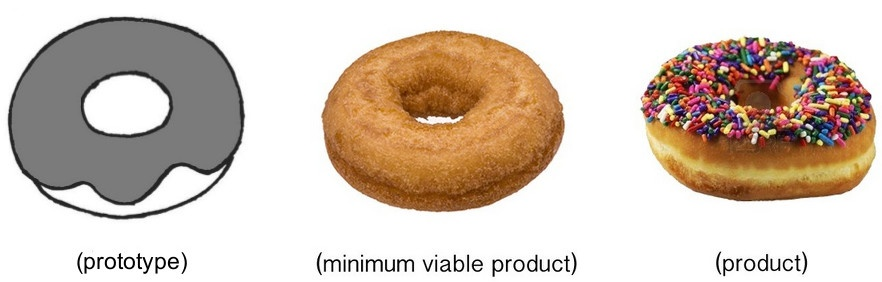
\includegraphics[width=10cm]{prototype-mvp-product.jpg}
\caption{Prototype, MVP and Product}
\label{fig:mvp-pic} %%% a label allows you to reference the figure in the text
%\medskip
\small
\end{figure}

This development technique is applicable to data projects as well because one can hardly expect their first product would be the perfect one for its first try. This minimum but working product will enable your team and client to test the basic models and analyses so that the further development and improvement of your product become easier and faster.

For your understanding, these short articles from industry data scientists will be helpful: \href{https://medium.com/idealo-tech-blog/what-is-minimum-viable-data-product-49269e338d85}{What is Minimum Viable (Data) Product?} by Dat Tran, \href{https://venturebeat.com/2018/11/24/before-you-launch-your-machine-learning-model-start-with-an-mvp/}{Before you launch your machine learning model, start with an MVP} by Jennifer Prendki, and \href{https://blog.dataiku.com/mvp-for-data-projects}{MVP for Data Projects} by Lynn Heidmann. \cite{MVPforDP}  


% ------------------------------------------------------------
\subsection{Post-MVP features}
% ------------------------------------------------------------
Your MVP is a minimal (working) version of your product and analysis, so as soon as you show its viability, you should ask "What are the other features that you will add or improve?" 

Ask yourself questions like:
\begin{itemize}
    \item What if our MVP doesn't answer all the questions the client asked us?
    \item How can MVP be improved to answer the questions or to achieve the goals?
    \item Can additional features be introduced to better answer the questions or get to the goals?
\end{itemize}


% ------------------------------------------------------------
\subsection{Stretch goals}
% ------------------------------------------------------------
What features would be nice to have but are either not essential or are currently too challenging to implement?

% ------------------------------------------------------------
\section{Risks and solutions}
% ------------------------------------------------------------
   List up to top 5 potential problems that might hinder the successful delivery of the product in \textit{this phase}. 
   Order the risks from the most severe and likely to the least severe and/or least likely.
   Describe these problems, along with an approach for how they will be addressed / resolved.
   Use the following format:
   
   \subsection{Risk \#1}
   Describe the problem.
   
   \textbf{Potential Solution(s): }

   \subsection{Risk \#2}
   Describe the problem.
   
   \textbf{Potential Solution(s): }

% ------------------------------------------------------------
\section{Timeline}
% ------------------------------------------------------------
%%% Remove/comment-out these instructions before turning in your plan.
Outline a timeline for all phases. I suggest dividing your whole timeline into four phases in this plan.

Make sure to account for the project report, the final presentation, and the finished product as part of the deliverables at the last phase.
I recommend not planning any development during the last phase especially after code freeze.
% ------------------------------------------------------------
\subsection{Overview of Deliverables}
% ------------------------------------------------------------
%%% This is a summary of delivarables you propose to your client
Summary of Deliverables: 

\begin{enumerate}
   \item Phase 1
   \begin{itemize}
     \item ...
     \item ...
   \end{itemize}
   \item Phase 2
   \begin{itemize}
     \item ...
     \item ...
   \end{itemize}
   \item Phase 3
   \begin{itemize}
     \item ...
     \item ...
   \end{itemize}
   \item Phase 4
   \begin{itemize}
     \item ...
     \item ...
   \end{itemize}
\end{enumerate}


% ------------------------------------------------------------
\subsection{Phase 1: MM/DD/YYYY -- MM/DD/YYYY}
% ------------------------------------------------------------
% Phase 1 - Define Project: understand business problem, define analytical problem, define technical problem.
Briefly explain what the tasks, events, and deliverables would be for the Phase 1.

% ------------------------------------------------------------
\subsection{Phase 2: MM/DD/YYYY -- MM/DD/YYYY}
% ------------------------------------------------------------
% Phase 2 - Data Phase: acquire, prepare, and understand your data  
Briefly explain what the tasks, events, and deliverables would be for the Phase 2. This would be the end of mid-term presentation. 

% ------------------------------------------------------------
\subsection{Phase 3: MM/DD/YYYY -- MM/DD/YYYY}
% ------------------------------------------------------------
% Phase 3 - Modeling Phase: train, evaluate, and improve your model
Briefly explain what the tasks, events, and deliverables would be for the Phase 3.

% ------------------------------------------------------------
\subsection{Phase 4: MM/DD/YYYY -- MM/DD/YYYY}
% ------------------------------------------------------------
% Phase 4 - Deployment Phase: finalize, deploy, and feedback (report and presentation).
Briefly explain what the tasks, events, and deliverables would be for the Phase 4. This is your final phase. Make sure to add the project report, the final presentation, and the finished product.

\pagebreak


%%%%%%%%%%%%%%%%%%%%%%%%%%%%%%%%%%%%%%%%%%
% Appendix Section 
% Author: Bhaven Mistry 
% Date: February 2020
%%%%%%%%%%%%%%%%%%%%%%%%%%%%%%%%%%%%%%%%%%
%%% Appendices.

%%% For your Statement of Work, you probably won't have any
%%% appendices, but you could include some if you really needed to.

%%% The appendices are delineated with the \appendix command.
%%% Individual appendices are begun with the standard \chapter or
%%% \section commands.  In our example, we'll \include them just as we
%%% did other chapters.

%%% Even in a relatively short document such as your statement of
%%% work, you might need to have appendices.  If so, uncomment
%%% the \appendix command and add them below (remember, the
%%% top-level structural command in this format is section).

\appendix

%%% DELETE THIS SECTION 
%%% This section is to give you some examples
\section{Useful \LaTeX ~examples} 
 
\subsection{Text styling}
An example of how to \texttt{create text} that is \textbf{bold} or \textit{italicized}. 

\subsection{Figures}
This is how you reference a figure (see Figure~\ref{fig:universe-pic}).

\begin{figure}[h]
\centering
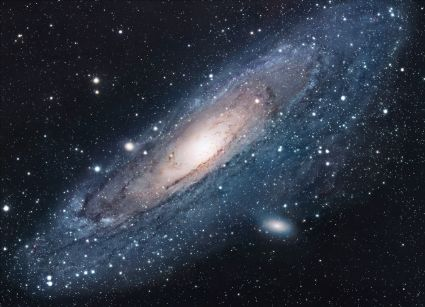
\includegraphics[width=0.15\textwidth, width=0.35\textwidth]{universe.jpg}
\caption{An example of an image with the corresponding caption.}
\label{fig:universe-pic} %%% a label allows you to reference the figure in the text
%\medskip
\small
\end{figure}

\subsection{References} 
An example of how to include a reference (\cite{OpenCV} and \cite{SIFT}) from you \texttt{.bib} file. Here's another way to reference something, which automatically adds parentheses around the citation~\citep{adams1995hitchhiker}.



%%% Bibliography.

%%% BibTeX is the tool to use for citations and layout of your
%%% bibliography.  Instead of having to type ``[5]'' or ``(Jones,
%%% 1968)'' (and keep track of which citation is which and renumber
%%% them as you add more references to your bibilography), you use
%%% special commands that allow BibTeX and LaTeX to automatically put
%%% the correct information in the right place.

%%% Section 5.6 in _The Mathematics Clinic in Brief: A Handbook_,
%%% talks about using BibTeX to format your bibliography and
%%% citations.

%%% Depending on your field, it may or may not be appropriate to list
%%% references for which you haven't included specific citations.  If
%%% your field sanctions such practices, or if you just want to get an
%%% idea of what you have in your bibliography file, you can include
%%% everything with the \nocite{*} command.
\nocite{*} 


%%% The appearance of your bibliography and citations in your text are
%%% defined by a combination of any bibliography-related LaTeX
%%% packages (such as natbib, harvard, or chicago) and the particular
%%% bibliography style file that you load with the \bibliographystyle
%%% command.  Bibliography-style files end in .bst; you can find them
%%% by searching your file system using whatever tools you have for
%%% doing searches.  (On most modern Unices, ``locate .bst'' will give
%%% you an idea of what's available.)

\bibliographystyle{acm}

%%% The particular bibliography data file or files that you want to
%%% use are specified with the \bibliography file.  Multiple files are
%%% separated by commas.

%%% You might want to use multiple bibliography (or ``bib'') files if
%%% you had a master bib file containing references you use again and
%%% again, and another containing only records for references for a
%%% particular project.

%%% Many people create a single, large bib file that they use for
%%% everything they write.  That approach requires you to \cite every
%%% reference that you want to use in your document -- using
%%% \nocite{*} with a huge bibliography database will give you a large
%%% bibliography containing many references you haven't consulted for
%%% your particular document!
\pagebreak

\bibliography{references}


%%% Glossary or Index.

%%% Having a glossary or index in a statement of work is overkill.
%%% Just define your terms in the text and you'll be fine.


\end{document}
